\documentclass[11pt]{article}
\usepackage{hyperref}
\usepackage{graphicx}
\usepackage{caption}
\usepackage{geometry}
\usepackage{float}
\usepackage{amsmath}
\usepackage{tikz}
\usetikzlibrary{shapes,arrows,positioning}
\usepackage{enumitem}
\usepackage{tabularx}

\geometry{a4paper, margin=1.5cm}
\setlength{\parindent}{0em}
\setlength{\parskip}{0.5em}

\begin{document}

\begin{titlepage}
    \centering
    \vspace*{1cm}

    % University Logo
    
\includegraphics[width=0.3\textwidth]{figures/ub_logo.png}

    \vspace{1.5cm}
    {\Huge\bfseries Sprint 1: Project Proposal\par}
    \vspace{1cm}
    {\large Procedurally Generated 2D RPG with AI-Driven Narrative\par}
    \vspace{2cm}
    {\large Oriol MIR\'O, Jean DI\'E, Bruno SANCHEZ, D\'aniel M\'ACSAI\par}
    \vspace{3cm}
    {\large \textbf{Master in Artificial Intelligence}\par}
    \vspace{0.5cm}
    {\large \textbf{Normative and Dynamic Virtual Worlds}\\ Sprint 1: Project Proposal\par}
    \vspace{1cm}
    {\large\bfseries October 7th, 2025\par}
\end{titlepage}

\pagestyle{empty}

\newpage
\tableofcontents
\newpage

% Set page numbering
\setcounter{page}{1}
\pagestyle{plain}

%% main text
\section{Introduction}
\label{sec:introduction}

Roguelike games have captivated players for decades with their promise of endless variety through procedural generation. Games like \emph{Enter the Gungeon} or \emph{Spelunky} demonstrate how algorithmically generated dungeons combined with intelligent enemy behaviours create highly replayable experiences.

Our project focuses on creating a 2D roguelike RPG where procedural content generation drives the core gameplay. 
The main challenge lies in algorithmically generating unique, playable dungeons for each playthrough while maintaining appropriate difficulty and player engagement. 
We will create a complete game where dungeon layouts are entirely procedurally generated, offering infinite replayability without requiring manual level design.

We aim to demonstrate the practical application of procedural content generation (PCG) techniques for dynamic level design. 
The roguelike structure provides an ideal framework: each playthrough tests whether our algorithms can consistently generate engaging, fair, and varied content without any hand-crafted level design.


\section{Scenario}
\label{sec:scenario}

\subsection{The Player's Journey}

Our goal is to create an experience that feels alive and unrepeatable. Each run should feel like uncovering a world that has never existed before—and will never exist again. Every room, enemy encounter, and story beat is generated specifically for the current playthrough, ensuring constant novelty and replayability. 

At the core of this vision lies a simple question: how can procedural generation sustain both challenge and meaning over time? We believe a \emph{checkpoint-based roguelike loop} combines permanence with variety. Players would progress through three major dungeon regions, each culminating in a unique boss (Figure~\ref{fig:game_flow}). Defeating a boss creates a checkpoint. 
Should the player fall, they return to the last checkpoint, but everything ahead is regenerated, reshaping both the level layout and narrative context. 

\begin{figure}[H]
    \centering
    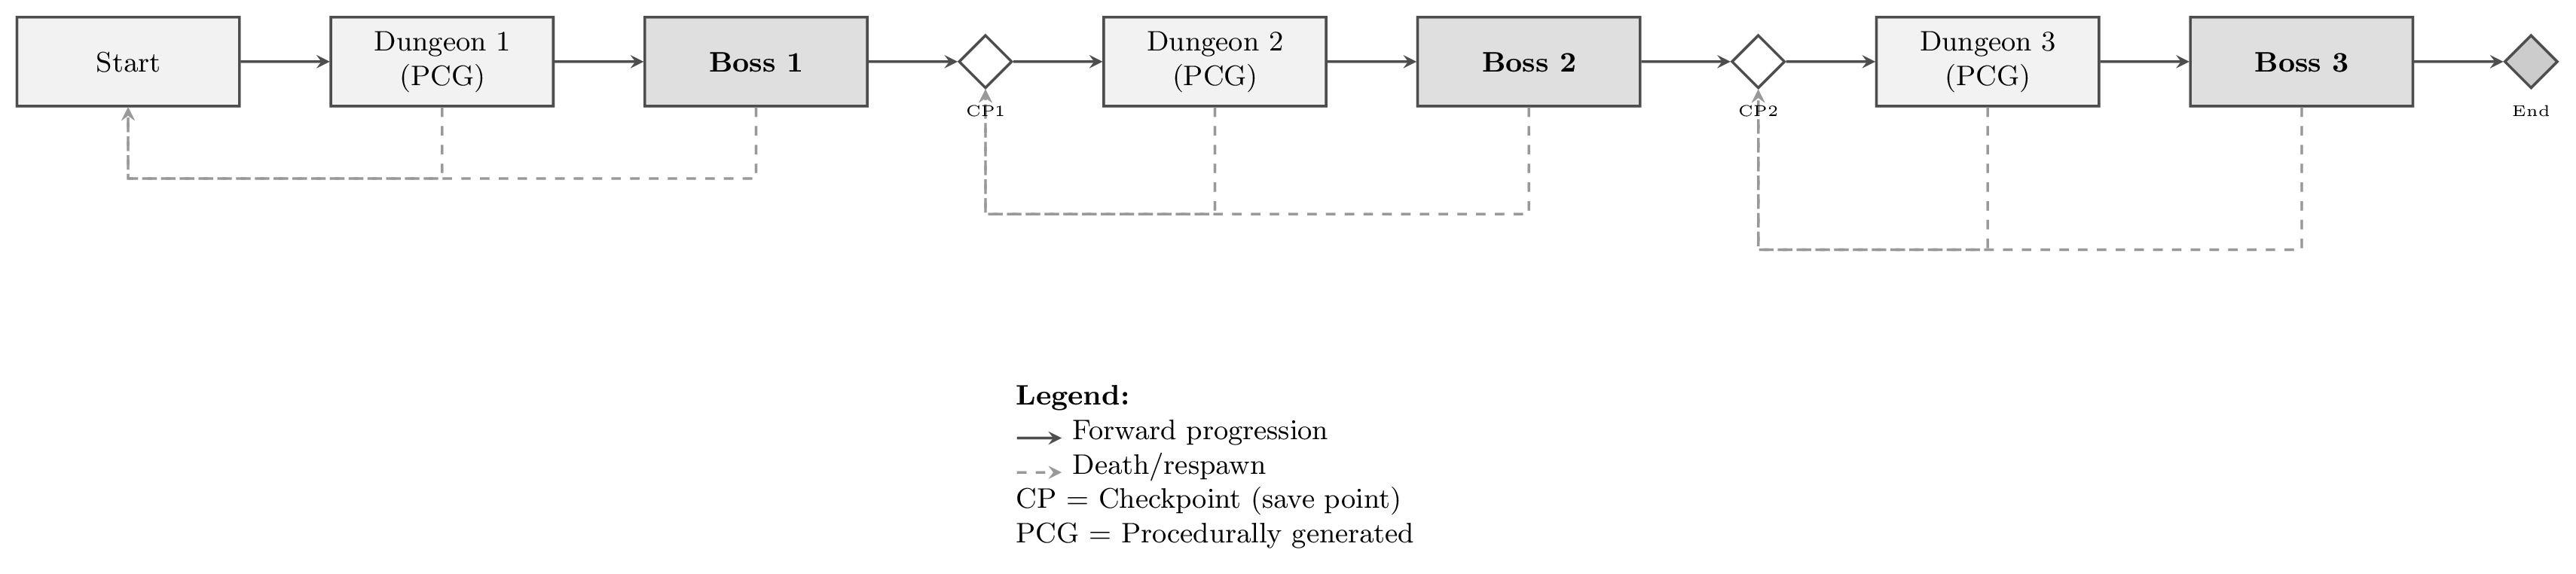
\includegraphics[width=0.8\textwidth]{figures/game_flow.png}
    \caption{The player's journey through three procedurally generated dungeon sections, each culminating in a boss fight that serves as a checkpoint. Death sends the player back to their last checkpoint, where both the dungeon and narrative regenerate.}
    \label{fig:game_flow}
\end{figure}

This structure naturally produces a rising difficulty curve. 
Early failures reset the run entirely -- harsh but motivating -- while later checkpoints offer meaningful progress and reduce frustration. 
The tension between risk and reward maintains engagement and reinforces the roguelike identity of the game.

We aim to produce a combat system akin to traditional RPGs: a health bar that depletes with each hit, encouraging players to master movement and timing. 
We're deliberately keeping these core mechanics straightforward to focus our development effort on the AI systems that make each encounter enjoyable rather than on complex combat mechanics.

Finally, we would like to see that aesthetic diversity supports the sense of progression. 
Each dungeon section should present a distinct visual and thematic identity: volcanic chambers, overgrown ruins, and crystalline caverns. 
This would also allow us to test different procedural generation parameters, ensuring that each stage feels mechanically and visually fresh.

\subsection{Progression and Potential LLM Integration}

The core progression follows a checkpoint-based system where defeating each boss creates a permanent save point. 
Beyond this structure, we're considering two optional features if development time permits.

A simple upgrade system could include coin collection and shops between sections, offering statistical improvements (health, damage, speed). 
The focus remains on getting core procedural generation working reliably.

As an experimental feature, we may explore LLM integration for dynamic narrative generation. 
This would involve feeding game state (current progress, bosses defeated) to an LLM to generate contextual story snippets.
While technically interesting, this remains secondary to our primary goal of robust procedural dungeon generation. 
If implemented, we'd use a simple approach: generate multiple options, select the most coherent, and tie narrative state to checkpoints.

\subsection{Game Agents}
\label{sec:game_agents}

Our focus in this project is \emph{procedural generation}; agent AI will be minimal and supportive. Following the course model, agents are specified as SENSE–THINK–ACT black boxes with simple components (navigation/physics, behaviour, animation) to keep implementation cost low.

As per the selected AI approach, for Sprint~1 we will use a compact \emph{Finite State Machine} (FSM) per enemy (idle/patrol $\rightarrow$ investigate $\rightarrow$ chase/attack $\rightarrow$ reset). 
This is lightweight, debuggable, and sufficient for showcasing PCG-driven encounters; a behaviour tree could be considered later if needed.

We do not yet know what enemies we might include, but some sketches are the following:
\begin{itemize}[leftmargin=1.2em,noitemsep]
  \item \textbf{Sentinel (melee grunt).} 
  \emph{Sense:} short-range vision cone, footstep noise. 
  \emph{Think:} FSM with alertness timer. 
  \emph{Act:} waypoint patrol, pathfind-to-player, simple swing attack. 
  \emph{State vars:} health, alertness, patrol\_index.
  \item \textbf{Spitter (ranged hazard).}
  \emph{Sense:} line-of-sight at medium range. 
  \emph{Think:} fire–cooldown cycle; strafe if player closes distance. 
  \emph{Act:} projectile volley, step-back, telegraphed reload. 
  \emph{State vars:} health, cooldown, preferred\_distance.
\end{itemize}

These two templates exercise the SENSE–THINK–ACT loop, basic navigation, and animation hooks without shifting focus away from level generation and checkpointed progression. They also let us validate difficulty profiling (spawn density, sight ranges, patrol graph) within generated layouts. 

\section{Related work}

Several commercial roguelikes and action platformers demonstrate viable patterns for combining procedural generation with authored constraints.

\textbf{Spelunky} popularised a hybrid, template-driven approach: hand-crafted ``room chunks'' are assembled into a grid with connectivity and placement rules (treasure, exits, hazards) to guarantee solvable, varied levels while retaining strong authored identity.

\textbf{Enter the Gungeon} drives level assembly from a \emph{flow graph}: a directed graph of room types and connections is sampled to define progression, loops, and special rooms (shops, boss antechambers), after which rooms are instantiated and spatially embedded.

\textbf{Unexplored} introduced \emph{cyclic dungeon generation}: designers specify high-level gameplay ``cycles'' (e.g., lock–key, shortcut, hub–spoke). The generator realises these dependencies in space to produce dungeons that feel hand-placed, with meaningful backtracking and pacing.

\textbf{Dead Cells} uses a hybrid of authored chunks and procedural stitching to achieve Metroidvania coherence: local constraints keep traversal rhythms and landmarks consistent while macro-scale randomisation preserves replayability.

These patterns inform our design choices: we prioritise \emph{structure-first} generation (graphs/constraints) combined with \emph{chunk-level variety} (templates/CA decoration) to balance reliability (connectivity, difficulty curves) and novelty (layout, encounters).


\section{Proposal}

\subsection{AI Design}
\label{sec:ai_techniques}

Procedural Content Generation (PCG) represents a family of algorithms that create game content algorithmically rather than manually. For 2D games, particularly roguelikes, PCG offers infinite replayability by generating unique levels, items, and encounters for each playthrough. This section surveys prominent PCG algorithms applicable to 2D game development, evaluating their strengths and use cases.

\subsubsection{Space Partitioning Algorithms}

\textbf{Binary Space Partitioning (BSP)} forms the foundation for structured level generation. The algorithm recursively subdivides rectangular space into smaller regions, places rooms within leaf nodes, and connects them with corridors. BSP excels at creating architectural layouts—dungeons, buildings, space stations—where rooms feel deliberately placed. Games like \textit{Spelunky} use BSP variants to ensure consistent level structure while varying room contents. The algorithm guarantees connectivity and offers fine control over room density, corridor width, and structural balance.

\textbf{Quadtree Partitioning} extends BSP by allowing non-uniform subdivisions. Rather than always splitting spaces in half, quadtrees can create four unequal child regions based on content requirements. This produces more organic variation in room sizes while maintaining the structured feel of partitioning algorithms. Quadtrees particularly suit games requiring hierarchical detail levels—larger combat arenas connected to smaller treasure rooms.

\subsubsection{Cellular Automata and Rule-Based Generation}

\textbf{Cellular Automata (CA)} generates organic, cave-like environments through iterative local rules. Each cell examines its neighbors and transitions between states (wall/floor) based on simple thresholds. Conway's Game of Life demonstrates this principle; for dungeon generation, typical rules convert cells to walls if surrounded by many walls, creating natural-looking caverns. CA requires minimal parameters yet produces complex, irregular spaces that feel hand-sculpted. Post-processing removes disconnected regions and smooths jagged edges.

CA variants include:
\begin{itemize}
    \item \textbf{Drunkard's Walk}: A moving agent carves paths through solid space, creating winding corridors and interconnected caves. Controlling walk length and branching probability yields varied topologies.
    \item \textbf{Diffusion-Limited Aggregation}: Particles randomly walk until encountering existing structure, then stick. This creates branching, tree-like level layouts resembling river deltas or root systems.
\end{itemize}

\subsubsection{Graph-Based Generation}

\textbf{Mission Graph Generation} treats levels as graphs where nodes represent rooms/encounters and edges represent connections. Designers specify high-level structure (e.g., "linear sequence with optional side branches") and the algorithm places rooms to match this topology. Graph-based PCG separates spatial layout from gameplay structure, enabling precise control over progression pacing, challenge curves, and optional content placement. \textit{Unexplored} uses cyclic graph generation to create lock-and-key puzzles with guaranteed solutions.

\textbf{Wave Function Collapse (WFC)} generates levels by satisfying local constraints. Given tile patterns and adjacency rules, WFC iteratively collapses superpositions (possible tile choices) to valid configurations. The algorithm ensures visual coherence—brick walls only connect to compatible tiles—while producing organic variety. WFC excels at generating levels that match hand-crafted aesthetic quality, though it's computationally expensive and can fail to converge without careful constraint design.

\subsubsection{Grammar-Based and L-Systems}

\textbf{L-Systems} use rewriting rules to generate complex structures from simple axioms. Originally designed for modeling plant growth, L-Systems apply to dungeon generation by treating level elements as symbols. For example, "C $\rightarrow$ C+R-C" might mean "a corridor branches into a room then continues." Successive rule applications create intricate, self-similar level topologies. L-Systems provide compact representation of complex structures and naturally create themed variations by modifying rule sets.

\textbf{Grammar-Based PCG} generalizes L-Systems using formal grammars. Non-terminal symbols represent abstract concepts (e.g., "combat area," "puzzle section") that expand into concrete implementations. This enables hierarchical generation: high-level narrative structure generates mid-level room sequences that finally instantiate as specific layouts. Grammar-based approaches excel at maintaining design coherence across scales.

\subsubsection{Noise Functions and Heightmap-Based Generation}

\textbf{Perlin/Simplex Noise} generates smooth, continuous random fields useful for terrain generation. Thresholding noise values creates landmasses, water bodies, and elevation changes. Multiple octaves (frequencies) of noise layered together produce naturalistic terrain with both large features and fine detail. While primarily used for outdoor/terrain generation, noise functions can define dungeon density maps—high noise values become dense wall clusters, low values open chambers.

\textbf{Voronoi Diagrams} partition space based on distance to seed points, creating irregular polygonal regions. Each region becomes a room or zone, with shared boundaries suggesting natural connection points. Voronoi generation produces more organic room shapes than BSP while maintaining clear spatial organization. Adjusting seed distribution (uniform, clustered, Poisson-disc) controls room size variation.

\subsubsection{Hybrid Approaches}

Modern PCG systems combine multiple algorithms to leverage complementary strengths:

\begin{itemize}
    \item \textbf{BSP + CA}: BSP creates overall structure; CA decorates rooms with organic details (rubble, vegetation, water pools).
    \item \textbf{Graph + WFC}: Mission graphs define gameplay flow; WFC fills graph nodes with visually coherent room layouts.
    \item \textbf{Grammar + Noise}: Grammars generate high-level structure; noise functions add environmental variation and decorative elements.
\end{itemize}

\subsubsection{Validation and Quality Assurance}

Regardless of generation algorithm, PCG systems require validation to ensure playability:

\begin{itemize}
    \item \textbf{Connectivity Analysis}: Graph algorithms (BFS/DFS) verify all areas are reachable. Unreachable regions are removed or connected.
    \item \textbf{Difficulty Profiling}: Simulations or heuristics estimate challenge level. Rooms with excessive enemy density or insufficient resources are rejected.
    \item \textbf{Solution Verification}: For puzzle-focused games, validators confirm intended solutions exist and unintended shortcuts don't trivialize challenges.
    \item \textbf{Aesthetic Constraints}: Pattern detection removes visually unappealing artifacts (e.g., single-tile gaps, excessively thin walls).
\end{itemize}

\subsubsection{Selected Algorithms for Our Project}

For our roguelike implementation, we will focus on two complementary approaches:

\textbf{Cellular Automata} for organic cave systems emphasizing exploration and environmental storytelling. CA's simplicity enables rapid iteration while producing naturalistic environments.

\textbf{Binary Space Partitioning} for structured dungeon sections emphasizing combat and tactical positioning. BSP's predictability ensures fair encounters while room variation maintains interest.

This combination provides aesthetic variety (caves vs. fortresses), supports different gameplay modes (exploration vs. combat), and demonstrates both rule-based and space-partitioning paradigms. Validation systems will ensure connectivity, appropriate difficulty progression, and fair player challenges across both generation methods.

\section{Implementation Plan}
\label{sec:technical}

\subsection{Development Platform}

We'll use \textbf{Unity 2D} for its mature 2D development tools, extensive asset store for graphics, and strong component-based architecture that suits modular AI implementation. This lets us focus on AI systems rather than building basic game infrastructure.

\subsection{Team Roles}
\begin{itemize}
    \item \textbf{Manager:} Oriol Miró - Coordination, integration, deliverables
    \item \textbf{AI Designer:} Dániel Mácsai - Level design, game balance, enemy placement
    \item \textbf{AI Tech:} Jean Dié \& Bruno Sanchez - Procedural generation algorithms, validation systems
\end{itemize}


%% Authors are advised to submit their bibtex database files. They are
%% requested to list a bibtex style file in the manuscript if they do
%% not want to use model1-num-names.bst.

%% References without bibTeX database:

% \begin{thebibliography}{00}

%% \bibitem must have the following form:
%%   \bibitem{key}...
%%

% \bibitem{}

% \end{thebibliography}


\end{document}

%%
%% End of file `elsarticle-template-1-num.tex'.